%%%% Paramétrage du cours %%%%
\def\xxactivite{Cours}
\def\xxauteur{\textsl{Xavier Pessoles}}

\fichefalse
\proftrue
\tdfalse
\courstrue

\def\xxnumchapitre{Chapitre 1 \vspace{.2cm}}
\def\xxchapitre{\hspace{.12cm} Introduction aux méthodes numériques}

\def\xxcompetences{%
\textsl{%
\textbf{Savoirs et compétences :}\\
\begin{itemize}[label=\ding{112},font=\color{ocre}] 
\item B2-12 : proposer un modèle cinématique à partir d'un système réel ou d'une maquette numérique;
\item B2-15 : Simplifier un modèle de mécanisme.
\end{itemize}
}}


\def\xxfigures{
\includegraphics[width=0.6\textwidth]{lola}\\
\textit{Robot humanoïde Lola}

\vspace{.5cm}

\includegraphics[width=0.5\textwidth]{simu}\\
%\textit{Simulateur de vol Lockheed Martin}
}%figues de la page de garde%figues de la page de garde

\input{\repStyle/new_pagegarde}
\vspace{2cm}
\pagestyle{fancy}
\thispagestyle{plain}


\section{Equations stationnaires}

\section{Intégration numérique}

\begin{hypo}  $f:[a,b]\rightarrow \mathbb{R}$ est une fonction continue sur $[a,b]$. On note $I = \int\limits_a^{b} f(x) \mathrm{d}x $.
\end{hypo}

\subsection{Principe des méthodes des rectangles}
%\subsection{Principe}
\begin{defi}
Dans cette méthode, la fonction à intégrer est interpolée par un polynôme de degré 0, à savoir une fonction constante. Géométriquement, l'aire sous la courbe est alors approximée par un rectangle. Plusieurs choix sont possibles.

\begin{minipage}[c]{.3\linewidth}
Rectangles à gauche :

$$
I = \int\limits_a^{b} f(x) \mathrm{d}x \simeq \left(b-a\right) f(a) 
$$
\end{minipage}\hfill
\begin{minipage}[c]{.3\linewidth}
Point milieu :

$$
I = \int\limits_a^{b} f(x) \mathrm{d}x \simeq \left(b-a\right) f\left(\dfrac{a+b}{2}\right) 
$$
\end{minipage}\hfill
\begin{minipage}[c]{.3\linewidth}
Rectangles à droite :

$$
I = \int\limits_a^{b} f(x) \mathrm{d}x \simeq \left(b-a\right) f(b) 
$$
\end{minipage}
\end{defi}

\subsection{Interprétation graphique}

\begin{minipage}[c]{.24\linewidth}
\begin{center}
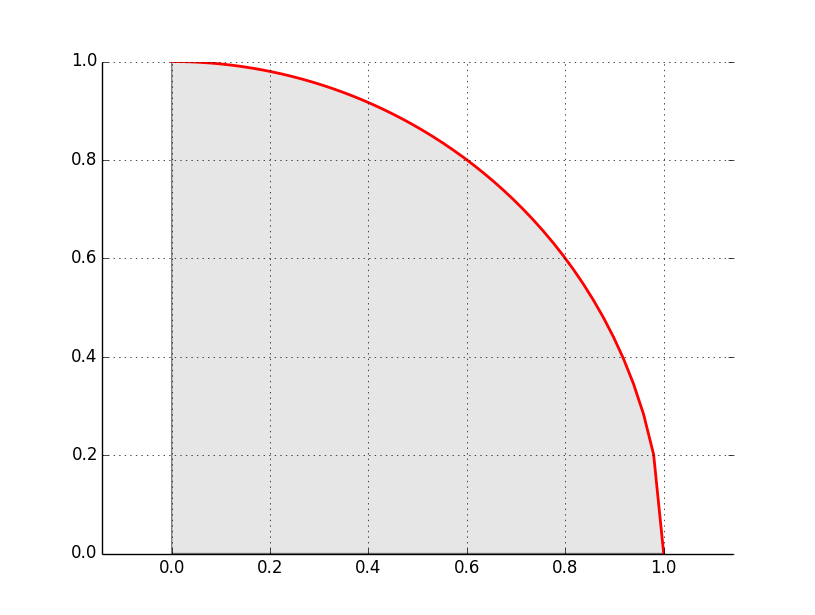
\includegraphics[width=.99\textwidth]{pi_courbe}

\textit{Calcul intégral}
\end{center}
\end{minipage}\hfill
\begin{minipage}[c]{.24\linewidth}
\begin{center}
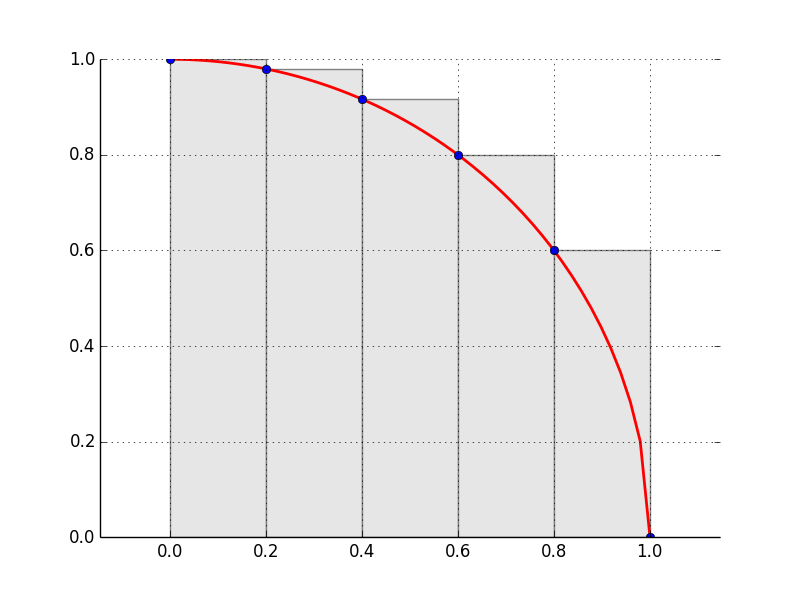
\includegraphics[width=.99\textwidth]{pi_rect_g}

\textit{Rectangles à gauche}
\end{center}
\end{minipage}\hfill
\begin{minipage}[c]{.24\linewidth}
\begin{center}
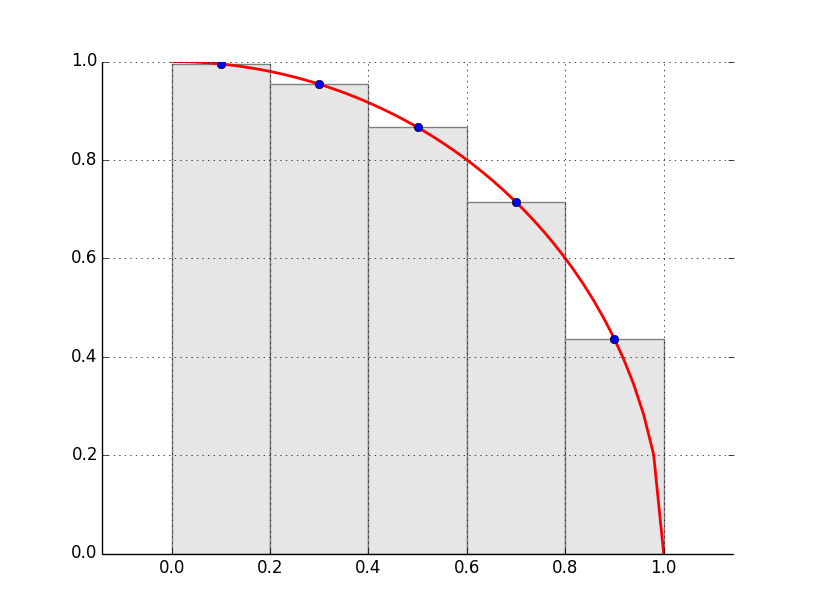
\includegraphics[width=.99\textwidth]{pi_rect_m}

\textit{Point milieu}
\end{center}
\end{minipage}\hfill
\begin{minipage}[c]{.24\linewidth}
\begin{center}
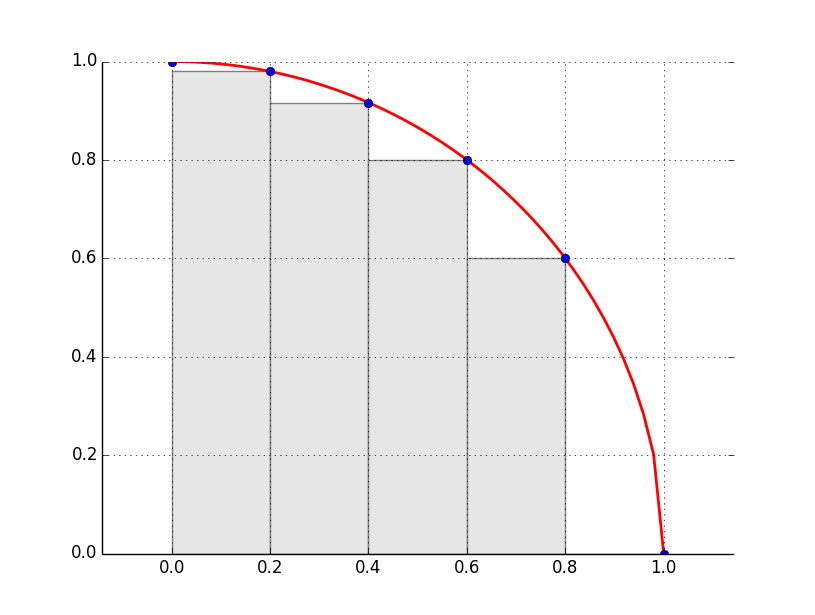
\includegraphics[width=.99\textwidth]{pi_rect_d}

\textit{Rectangles à droite}
\end{center}
\end{minipage}


\subsection{Principe des méthodes des trapèzes}
\begin{minipage}[c]{.7\linewidth}
\begin{defi}
Dans cette méthode, la fonction à intégrer est interpolée par un polynôme de degré 1, à savoir une fonction affine. Géométriquement, l'aire sous la courbe est alors approximée par un trapèze :

$$
I = \int\limits_a^{b} f(x) \mathrm{d}x \simeq \left(b-a\right) \dfrac{f(a)+f(b)}{2} 
$$
\end{defi}
\end{minipage}\hfill
\begin{minipage}[c]{.24\linewidth}
\begin{center}
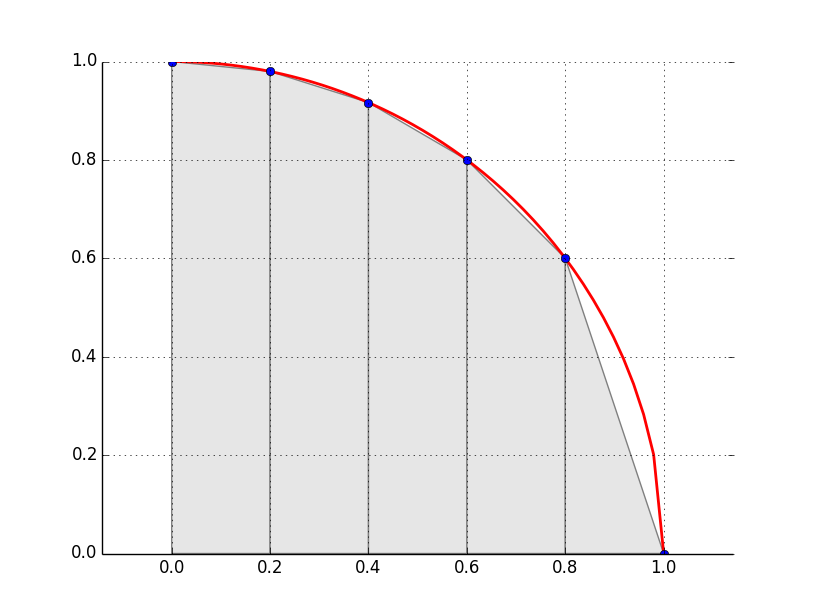
\includegraphics[width=.99\textwidth]{pi_trap}
\end{center}
\end{minipage}

\subsection*{Notion d'erreur d'intégration}
\begin{resultat}
Dans chaque cas,  on intègre $f$ sur $n$ subdivisions régulières de $I$. 

\textbf{Erreur sur la méthode des rectangles à gauche et à droite}

Soit $f$ fonction dérivable sur $I=[a,b]$ et dont $f'$ est continue sur $I$. Soit $M_1$ un majorant de $f'$ sur $I$. L'erreur $\varepsilon$ commise lors de l'intégration par la méthode des rectangles à droite ou à gauche
 est telle que $ \varepsilon \leq \dfrac{M_1}{2n}$.

\textbf{Erreur sur la méthode des rectangles -- point milieu}

Si de plus $f$ est deux fois dérivables sur $I=[a,b]$ et $f''$ est continue sur $I$, on note $M_2$ un majorant de $f''$ sur $I$.L'erreur $\varepsilon$ commise lors de l'intégration par la méthode des rectangles -- point milieu est telle que $ \varepsilon \leq \dfrac{M_2}{12n^2}$.

\textbf{Erreur sur la méthode des trapèzes}

L'erreur commise$\varepsilon$ est telle qu'il existe un entier $M$ tel que $ \varepsilon \leq \dfrac{M}{12n^2}$.

\end{resultat}
\newpage

\subsection*{Bibliothèque Python}
Il est possible d'intégrer une fonction en utilisant les modules de la bibliothèque \texttt{scipy} :
\begin{lstlisting}
from scipy.integrate import quad
from math import sin
# Définition des bornes de gauche et de droite
g,d = -1,1 
def f(x):
    return sin(x)
   
I,erreur = quad(f,g,d)
print(I,erreur)
\end{lstlisting}


\section{Résolution d'équations différentielles}

\section{Résolution de systèmes linéaires}
